%!TEX root = ../Thesis.tex
%\chapter{Long chapter title with $\pi$ $π$ or π}
%\chapter{Long chapter title with \texorpdfstring{$\pi$ $π$ or π}{π π or π}}
\chapter{Deep learning seismic facies on state of the art CNN architectures}

We explore propagation of seismic interpretation by deep learning in stacked 2D sections. We show the application of state-of-the-art image classification algorithms on seismic data. These algorithms were trained on big labeled photograph databases. We use transfer learning to benefit from pre-trained networks and evaluate their performance on seismic data.

{\vfill\hfill\newline\fbox{\parbox{.97\textwidth}{\fullcite{dramsch2018deep}}}}

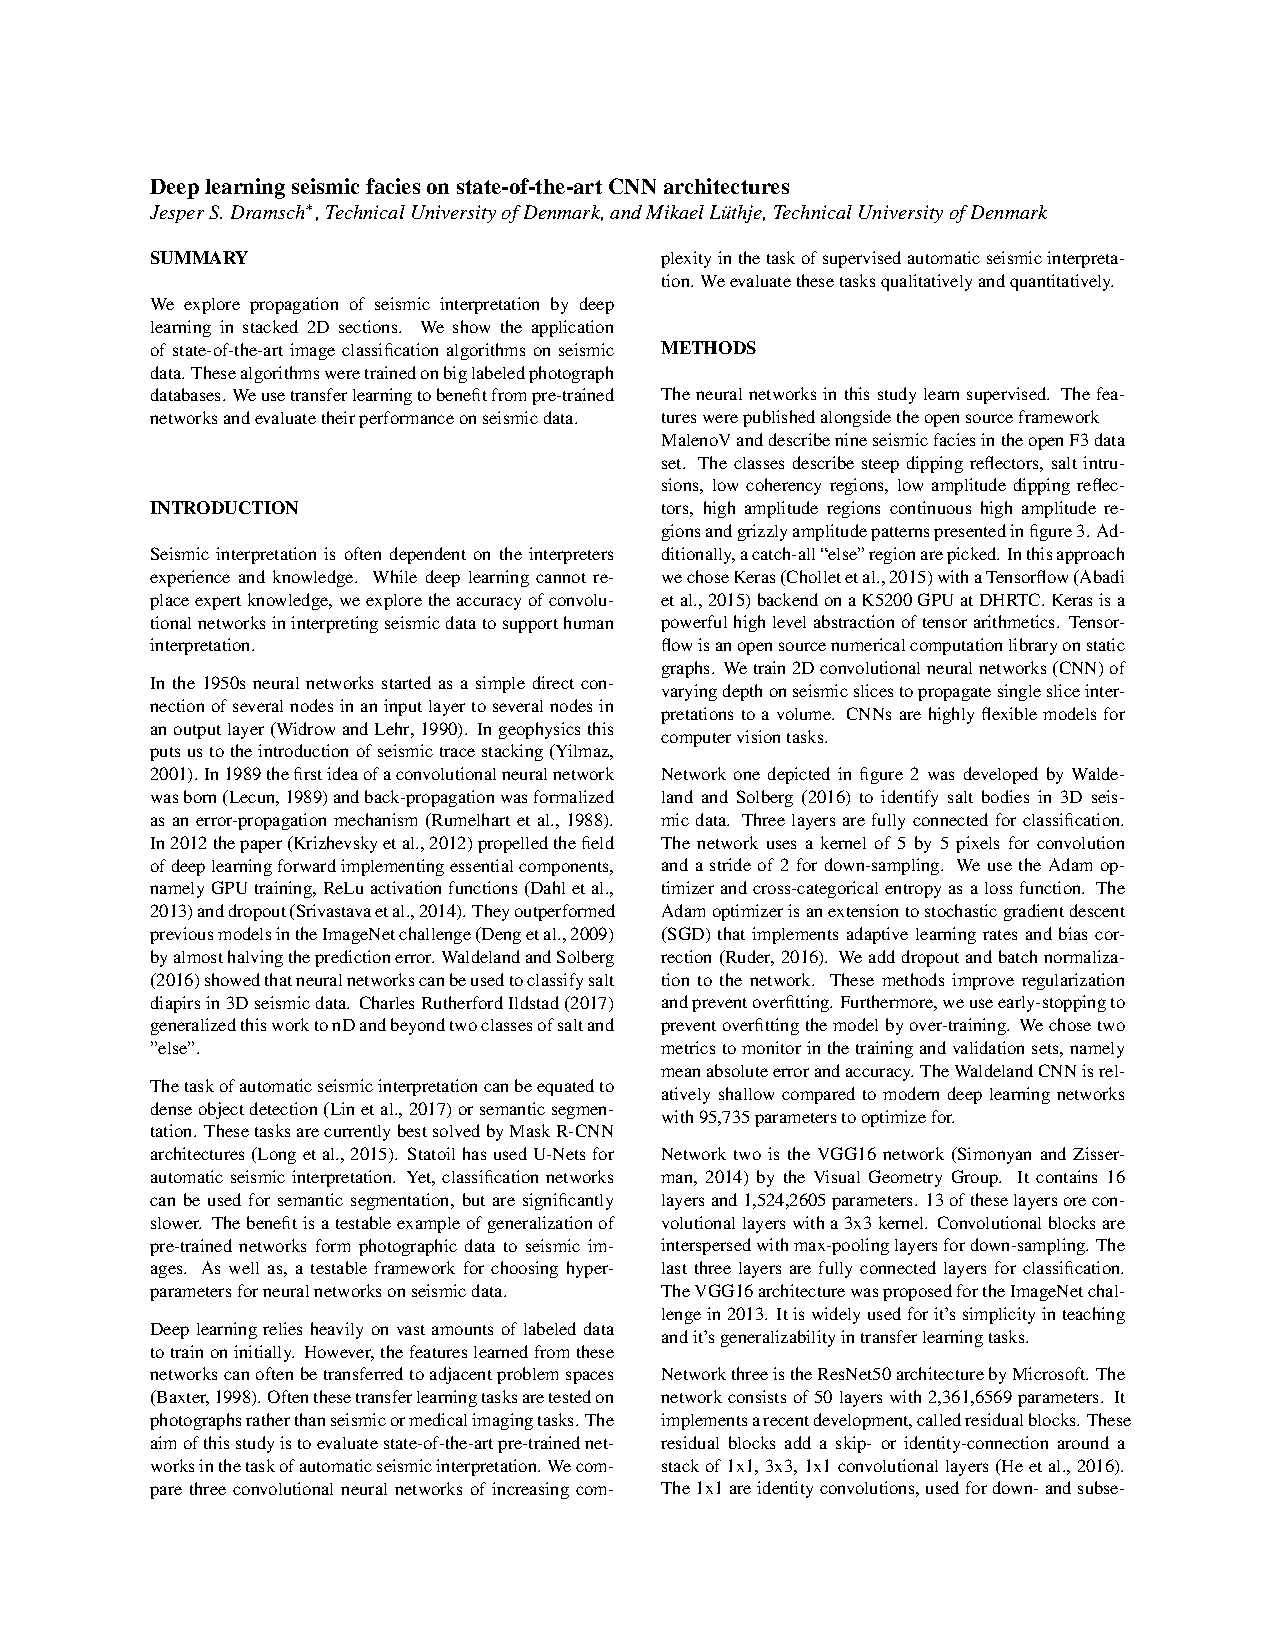
\includepdf[pages=1-4,pagecommand={},width=1.2\textwidth,offset=0.7cm -1.5cm]{papers/2018.4}
\todo{Check Page Numbers}
\todo{Fix Alignment}